\documentclass[man,floatsintext]{apa6}
\usepackage[nodoi]{apacite}
\usepackage{graphicx}
\usepackage[american]{babel}
\usepackage{amsmath}
\usepackage{enumitem}
\usepackage[section]{placeins}
\usepackage{subfigure}

\title{Adults and preschoolers flexibly adapt to noisy linguistic input}
\author{Daniel Yurovsky, Sarah Case, and Michael C. Frank}
\affiliation{Stanford University}
\shorttitle{Noisy Kids}
\leftheader{Yurovsky \& Frank}


\abstract{
}

\keywords{Language processing, noisy channel, cognitive development}

\authornote{Please address correspondence to: 

\vspace{12 pt}
Daniel Yurovsky

Jordan Hall (Building 420)

Stanford University

450 Serra Mall

Stanford, CA 94305

\vspace{12 pt}
Email: yurovsky@stanford.edu 

\vspace{24 pt}

Word Count: 
}

\begin{document}
\maketitle

Imagine Bob heard Alice say ``I had carrots and bees for dinner.'' Perhaps she visited an exotic restaurant, and he should follow up and ask how they tasted. Or perhaps he misheard her, or she misspoke. Interpreting her utterance requires integrating perceptual information about what he heard with his expectations: about both what words usually go with ``carrots'' and ``dinner'' and also what foods people usually eat. Statistical language processing systems operate using a body of theory based on this idea---that language is a \emph{noisy channel}, and that Bob can correct for perceptual errors using linguistic expectations about what Alice was likely trying to say \cite{jelinek1976, shannon1948}. 

Noisy channel principles provide a powerful framework for explaining how the human language processing system operate in complex and uncertain real-time communicative situations \cite{clayards2008, levy2008, jaeger2010, kleinschmidt2015}. On this view of human language, comprehenders integrate prior expectations with perceptual data; and they do so probabilistically, weighting each according to its reliability. In one demonstration of this sort of integration, \citeA{gibson2013} presented participants with semantically implausible sentences (e.g., ``The mother gave the candle the daughter''), which could have been produced by small typographical errors in otherwise much more plausible sentences (e.g., the omission of the word ``to''). Adult comprehenders were able to correct these errors, and they corrected them at especially high rates when they had reason to believe that the communicative channel was noisy (and hence the perceptual signal was unreliable). They also corrected these errors at lower rates when they believed they were in a ``silly'' context where many of the sentences they read were similarly implausible. Together, these manipulations suggested a flexible weighting on the perceptual signal---how noisy is the channel?---and prior expectations---how plausible is the speaker?.

Is children's language comprehension rooted in the same kind of flexible, expectation-based processing? 

% If we hear someone say that they ``had carrots and \emph{bees} for dinner,'' when should we rely on our perceptual signal, and when should we instead privilege our expectation that the speaker probably doesn't like to eat bees? If we are ideal observers, we should rely on each of these cues in proportion to their reliability \cite{ernst2002, jacobs1999}. For instance, if we are in a quiet room, and have additional bottom-up visual information from the speaker's mouth, we should be more likely to conclude that she said ``bees'' \cite{mcgurk1976}. On the other hand, if we are having trouble hearing because it is loud, or because we are speaking on a cell-phone which reduces the audio quality, we should be more inclined to think we misheard \cite{schroeder1985}. Similarly, if we have never met this speaker before, or know her to be serious and well-spoken, we should think ourselves to have misheard. But, if the speaker is our friend who we know to prone to being silly, we should be more likely to think we correctly heard ``bees.''

In the following experiments, we adapt \citeA{gibson2013}'s paradigm to test three novel predictions. First, we use a spoken language paradigm and a simpler model of noise (i.e. literally acoustic noise) to show that the same predictions hold in an environment more like daily language processing. Second, we show that listeners are sensitive to both of these manipulations in the same context, and adapt simultaneously to changing speaker expectations and noise levels. Third, we show that this flexible adaption occurs not only in adults, but also in preschool-aged children.

\begin{figure}[t]
     \begin{center}
     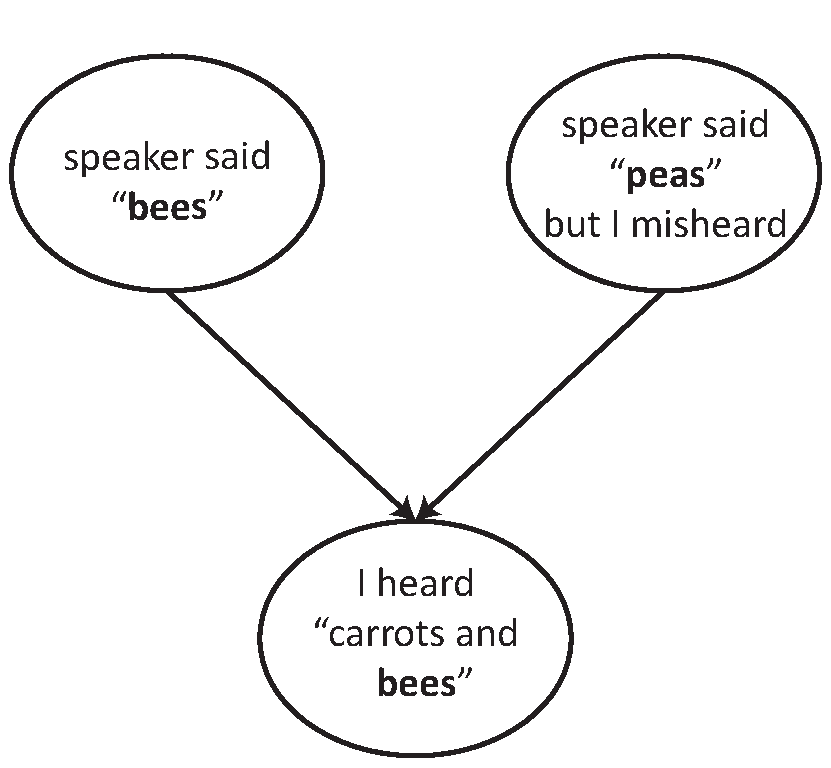
\includegraphics[width=0.5\textwidth]{figures/explaining_away.pdf}
    \end{center}
    \caption{Explaining away}%
   \label{fig:explaining_away}
\end{figure}

\section{Experiment 1}



\begin{figure}[t]
     \begin{center}
        \subfigure[]{
            \label{fig:training}
            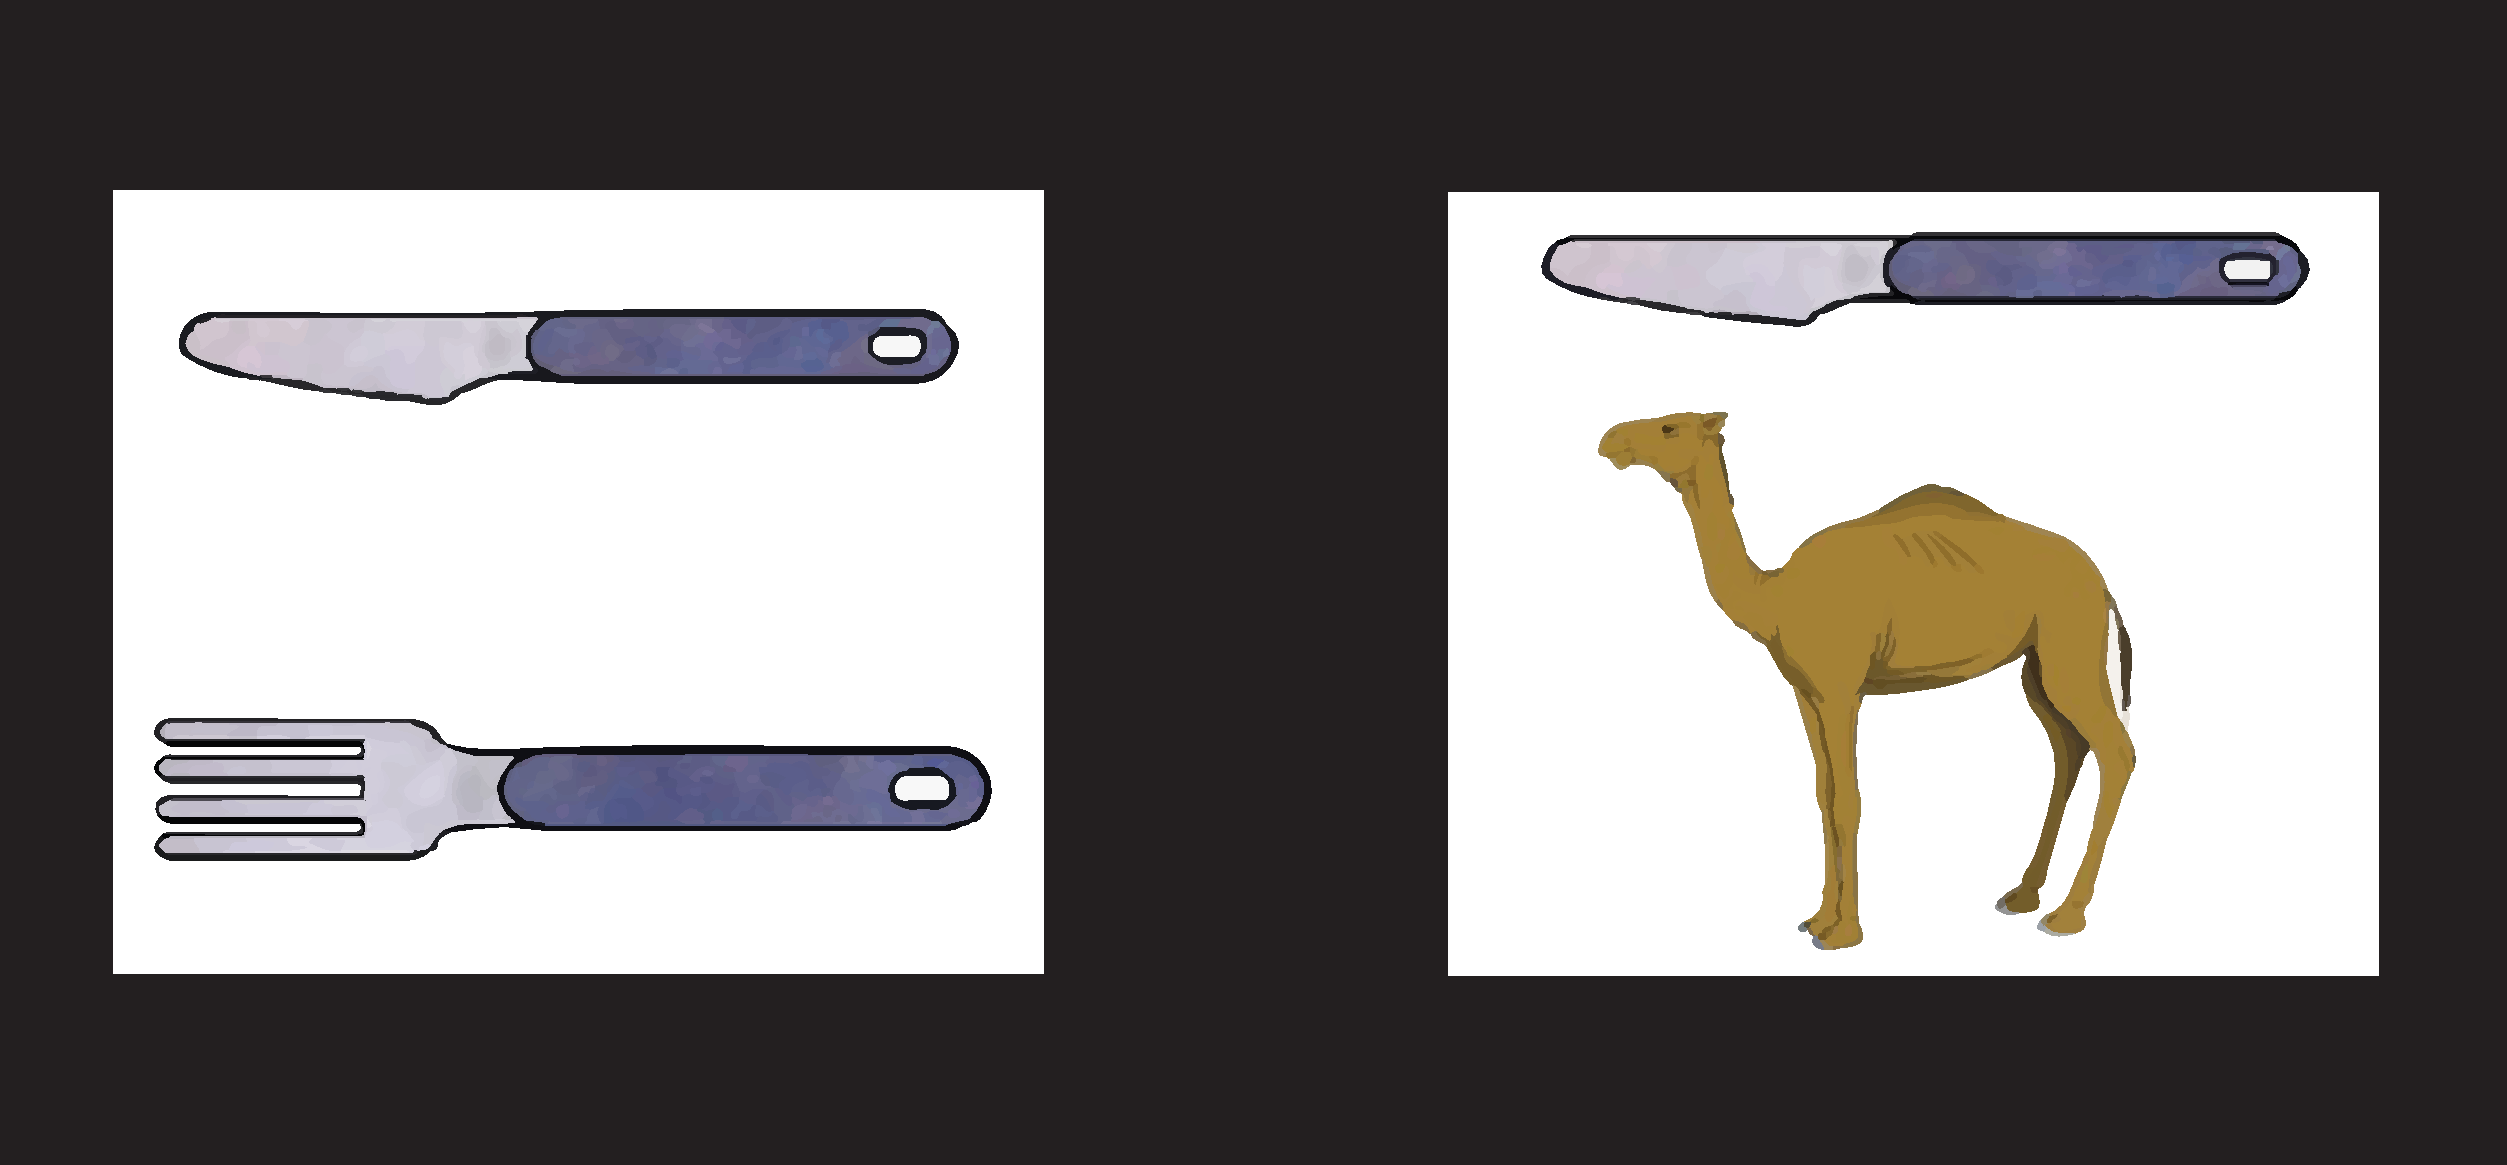
\includegraphics[width=0.4\textwidth]{figures/training.pdf}
        }
        \subfigure[]{
           \label{fig:testing}
           
\includegraphics[width=0.4\textwidth]{figures/testing.pdf}
        }
    \end{center}
    \caption{Training and test stimuli
     }%
   \label{fig:stimuli}
\end{figure}


\subsection{Method}
\subsubsection{Participants}

Adult participants for Experiment 1 were recruited through Amazon Mechnical Turk. We posted 50 Human Intelligence Tasks (HITs) to be completed only by participants with US IP addresses that each paid 30 cents. A total of 50 HITs were posted, with Speaker condition assigned randomly to each participant.

Children were recruited at the Bing Nursery School on Stanford's campus. Each child was asked if they would be willing to play a game with the experimenter, and informed that they could stop playing at any time. Children were randomly assigned to speaker conditions, and we collected data until there were at least 20 participants in each condition. Data from a total of 43 children was collected, Children were all between 4 and 6 years old, and approximately half were female. Neither age nor sex distribution varied significantly across conditions (Plausible: 23 children (12 girls), Mean age = 4.6 years (range = 4.0--5.3 years), Implausible: 20 children (10 girls), Mean age = 4.7 years (range = 4.1--5.4 years).

\subsubsection{Stimuli}

Stimuli for Experiment 1 were a series of screens on which participants saw two pictures and heard a sentence referring to one of them\footnote{All stimuli, as well as data and analyses are available in a public github repository at \small{\tt{http://github.com/dyurovsky/noisy-kids}}.} . The pictures were constructed from clipart freely available on the internet. Audio was recorded by a native English speaking female. 

\subsubsection{Procedure}

In each trial, participants saw two pictures on the screen, and heard a short sentence. Children saw two kinds of trials that manipulated the relationship of the pictures to each other. On introductory trials, children ... FIXME

\subsection{Results and Discussion}

In order to establish that both children and adults understood the task, and encoded the differences between the Plausible and Implausible speakers, we first analyze their performance on exposure trials. First, we ask whether participants selected the plausible referent when it was asked for by the Plausible speaker, and selected the implausible referent when it was asked for by the Implausible speaker. We submitted performance for each group and condition separately to a mixed-effects logistic regression with random effects of subject and trial. Both children and adults were significantly more likely to choose the plausible referent in the Plausible condition ($\beta_{adult} = 5.66$, $z = 6.76$, $p <.001$; $\beta_{child} = 2.62$, $z = 5.43$, $p <.001$), and significantly less likely than chance to choose the plausible referent in the Implausible condition ($\beta_{adult} = -3.87$, $z = -7.13$, $p <.001$; $\beta_{child} = -1.9$, $z = 5.61$, $p <.001$). To test the difference between the conditions directly, we further fit a mixed-effects regression predicting choice on Exposure trials from group, condition, and their interaction, and found significant effects of all three ($\beta_{child} = 1.96$,  $z = 3.33$, $p <.001$, $\beta_{Plausible Speaker} = 9.52$,  $z = 7.87$, $p <.001$,  $\beta_{group x condition} = -5$,  $z = -4.12$, $p <.001$). Thus, both children and adults were sensitive to the speaker manipulation during Exposure trials, selecting the appropriate referent whether or not the request was implausible, although adults showed a greater sensitivity to the manipulation.

\begin{figure}[t]
     \begin{center}
     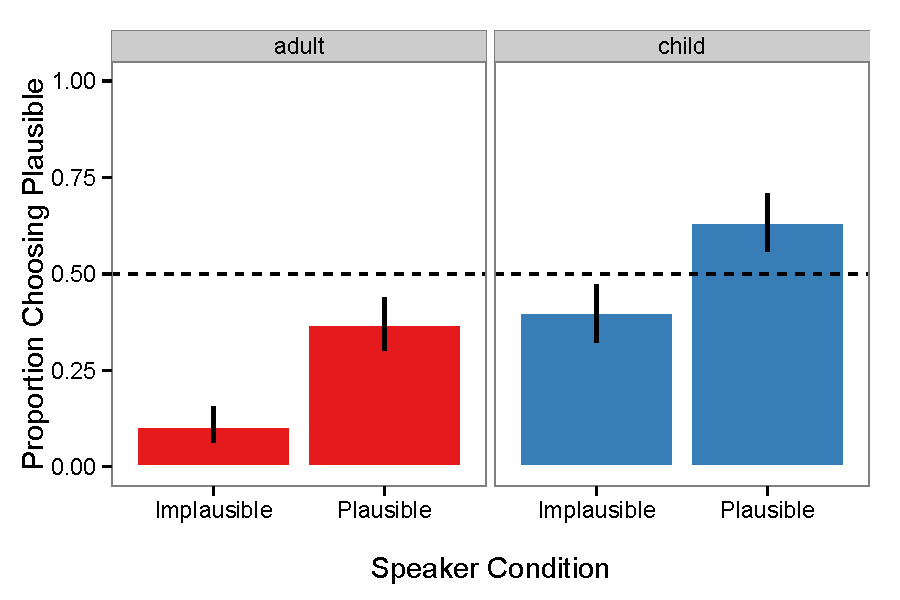
\includegraphics[width=0.5\textwidth]{figures/exp1_results.pdf}
    \end{center}
    \caption{Explaining away}%
   \label{fig:exp1_results}
\end{figure}

Did this exposure to a Plausible vs. Implausible speaker change participants' expectations during the ambiguous test trials? Figure~\ref{fig:exp1_results} shows the proportion of both children and adults who selected the plausible referent at test in both conditions. As predicted, both groups were sensitive to the manipulation, selecting the plausible referent more often in the Plausible Speaker condition. However, while children children were overall more likely to pick the plausible referent in both conditions, the size of the difference between conditions was comparable across adults and children, indicating a similar sensitivity to the speaker's prior productions. To confirm these findings formally, we again fit a mixed effects regression predicting choice on test trials from group (child vs. adult), condition (Plausible vs. Implausible Speaker), and their interaction. Both of the main effects were significant, but the interaction was not, indicating that both children and FIXME ($\beta_{child} = 1.96$,  $z = 3.33$, $p <.001$, $\beta_{Plausible Speaker} = 2.33$,  $z = 4.40$, $p <.001$,  $\beta_{group x condition} = -1.01$,  $z = -1.53$, $p = .13$).

Taken together, these results show that both adults and children are sensitive to the past productions of a novel speaker, rapidly learning the kinds of things they are likely to say. Further, they use this information to alter their expectations about what this speaker will say, and they use these expectations when interpreting ambiguous. Intriguingly, children did not alter their expectations significantly less than adults, showing that they adapt their expectations quite rapidly. Children were, however, more likely overall to pick the plausible referent during ambiguous test trials, suggesting that they may have a larger bias to rely on their language models rather than the acoustic signal. This is consonant with other evidence showing significantly more noise in children's perceptual systems (CITES).

\section{Experiment 2}

NEED CONTROL CONDITIONS SO...

\subsection{Method}

\subsubsection{Participants}

Children for Experiment 2 were recruited from the floor of the San Jose Children's Discovery museum. An experimenter approached the child and parent and obtained informed consent before inviting both to enter a separate room in which the ipad and camera were set up. Data was collected from a total of 

 Normal condition -- 26 children, 12 girls, age: mean = 4.98, min = 4.02, max = 5.94; Implausible -- 24 children, 11 girls, age: mean = 5.01, max = 5.92, min = 4.01, Control --- 20 children, 11 girls, age: mean = 4.96, max = 5,91, min = 4.15, No Noise Normal = 21 children, 8 girls, age: mean = 4.89, max = 5.93, min = 4.1, No Noise Implausible --- 20 children, 12 girls, age: mean = 4.98, max = 5.83, min = 4. 
 
\subsubsection{Stimuli and Design}

Each trial of the experiment presented two pictures on the screen of the ipad, and played a short sentence Katie. Children saw two kinds of trials that manipulated the relationship of the pictures to each other. On introductory trials, children 

\subsubsection{Procedure}

The experimenter then instructed the child that they would be playing a game in which a speaker named Katie would tell the child about one of the pictures on the screen, and that they should touch the one to which she was referring. The child was then shown a picture of Katie and asked if they understood the game. After they assented, they proceeded through eight introductory trials and then eight test trials. 

\subsection{Results and Discussion}

As in Experiment 1, we first establish that children understood the task, and encoded the differences between the Plausible and Implausible speakers during Exposure trials. First, we ask whether participants selected the plausible referent when it was asked for by the Plausible speaker, and selected the implausible referent when it was asked for by the Implausible speaker independent of noise level. We submitted performance for each condition and noise level separately to a mixed-effects logistic regression with random effects of subject and trial. As before, children were more likely than chance to choose the plausible referent in the Plausible condition, but less likely than chance to choose the plausible referent when the speaker asked for the implausible referent (Implausible and Control).  

To test the difference between the conditions directly, we further fit a mixed-effects regression predicting choice on Exposure trials from group, condition, and their interaction, and found significant effects of all three ($\beta_{child} = 1.96$,  $z = 3.33$, $p <.001$, $\beta_{Plausible Speaker} = 9.52$,  $z = 7.87$, $p <.001$,  $\beta_{group x condition} = -5$,  $z = -4.12$, $p <.001$). Thus, both children and adults were sensitive to the speaker manipulation during Exposure trials, selecting the appropriate referent whether or not the request was implausible, although adults showed a greater sensitivity to the manipulation.



\begin{figure}[t]
     \begin{center}
     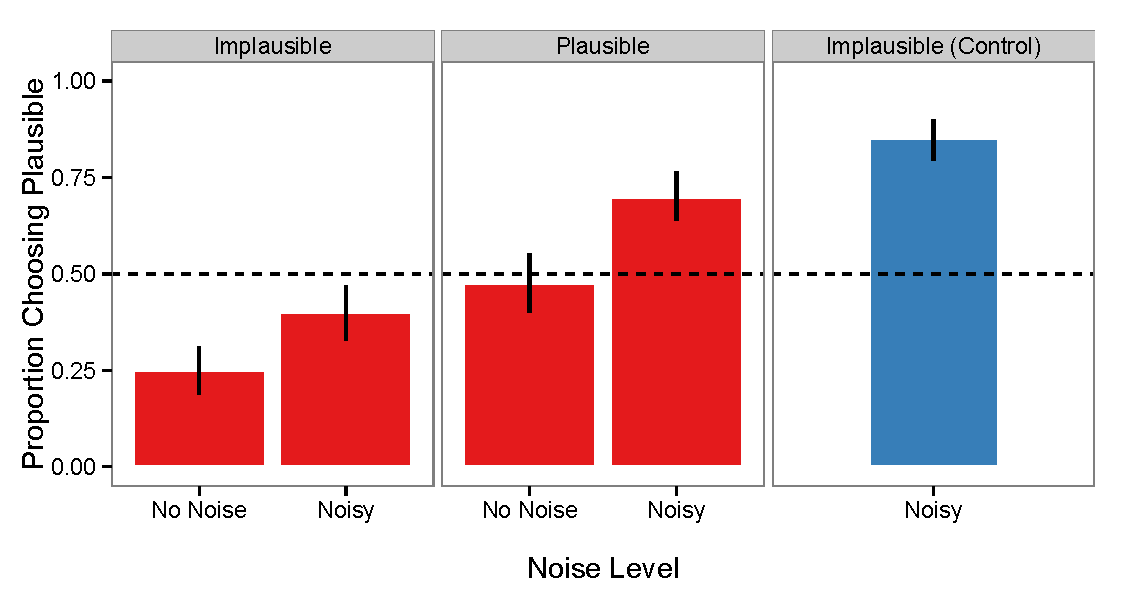
\includegraphics[width=0.5\textwidth]{figures/exp2_results.pdf}
    \end{center}
    \caption{Experiment 2 results}%
   \label{fig:exp2_results}
\end{figure}

\section{General Discussion}

\paragraph{From cue weighting to communicative inference}

\section{Acknowledgments}

We are grateful to Nicolette Castro for collecting the bulk of the child data, and all of the members of the Language and Cognition Lab for their feedback on this project. In addition, we thank the parents, children, and staff at the San Jose Children's Discovery Museum for supporting us in collecting developmental data. This work was supported by NIH NRSA F32HD075577 to DY as well as grants from the Merck Scholars Foundation and the Stanford Center Health Research Initiative to MCF.

\bibliographystyle{apacite}
\bibliography{noisy_kids}

\end{document}
